\chapter{Risultati ottenuti}

	Il sistema è stato avviato in locale, su un computer che funge sia da nodo \emph{master} che da nodo \emph{worker}.
	Al fine di analizzare le performance dei due sistemi (monolitico e a microservizi) è stato realizzato uno script che effettua mille ordini in successione.
	Le operazioni eseguite nel dettaglio sono le seguenti:
	
	\begin{enumerate}
		\item Viene selezionato in modo casuale un utente con il quale si effettua il login.
		
		\item Viene richiesta la lista articoli disponibili.
			Dalla lista vengono selezionati alcuni prodotti in modo casuale (da 1 a 15 prodotti diversi), ciascuno in quantità casuale tra 1 e 10;
			si genera così un carrello virtuale.
			
		\item Viene inviato l'ordine con i prodotti scelti.
		
		\item L'ordine viene pagato.
		
		\item Se non si sono generati errori la procedura è completata e si passa all'esecuzione della prossima iterazione.
	\end{enumerate}
	
	Ad ogni iterazione lo script memorizza l'intervallo di tempo in sei differenti punti:
	
	\begin{enumerate}
		\item Inizio della nuova iterazione.
		
		\item Completato il login dell'utente.
		
		\item Ottenuta la lista di prodotti dal server.
		
		\item Carrello riempito con i prodotti selezionati secondo la modalità precedentemente descritta.
		
		\item Il nuovo ordine è stato generato.
		
		\item Fine.
	\end{enumerate}
	
	Si possono quindi calcolare cinque intervalli di tempo, indicati in ordine con lettere da A ad E.
	In Tabella \ref{tab:tempi-monolitica} e \ref{tab:tempi-microserv} sono riportati gli indici statistici più rilevanti ottenuti dai dati inerenti i tempi di esecuzione di ogni fase, in Figura \ref{fig:grafici-monolitica} e \ref{fig:grafici-microserv} i dati sono invece rappresentati sotto forma di boxplot ed istogramma.

	L'indice di maggior interesse è sicuramente la media e si nota un generale leggero vantaggio per l'applicazione monolitica, dovuto al \emph{overhead} introdotto dall'orchestratore dei container.
	In un'applicazione molto semplice come quelle realizzate per questa ricerca la differenza è poco marcata o addirittura a
	Va anche tenuto in considerazione che il test è stato eseguito su un personal computer di potenza limitata, sicuramente ben lontano dalla capacità di calcolo offerta da un server reale.





	\begin{table}[tbp]
		\[
		\begin{array}{lccccc}
			\toprule
			\mbox{\textbf{Fase}} & \textbf{A} & \textbf{B} & \textbf{C} & \textbf{D} & \textbf{E}\\
			\midrule
			\mbox{Media} & 43.64 & 42.21 & 0.05 & 49.53 & 64.13\\
			\mbox{Minimo} & 29.74 & 30.36 & 0 & 35.69 & 30.81\\
			\mbox{1° quartile} & 38.23 & 37.44 & 0 & 43.62 & 37.0\\
			\mbox{Mediana} & 40.38 & 39.29 & 0 & 45.93 & 39.29\\
			\mbox{3° quartile} & 42.93 & 41.28 & 0 & 48.31 & 44.07\\
			\mbox{Massimo} & 208.61 & 170.06 & 1.54 & 179.83 & 271.9\\
			\bottomrule
		\end{array}
		\]
		\caption{Valori statistici ottenuti dall'esecuzione dell'applicazione monolitica. Tempi espressi in ms}
		\label{tab:tempi-monolitica}
	\end{table}
	
	\begin{table}[tbp]
		\[
		\begin{array}{lccccc}
			\toprule
			\mbox{\textbf{Fase}} & \textbf{A} & \textbf{B} & \textbf{C} & \textbf{D} & \textbf{E}\\
			\midrule
			\mbox{Media} & 44.06 & 44.15 & 0.06 & 62.84 & 7.64\\
			\mbox{Minimo} & 34.14 & 34.36 & 0 & 46.38 & 5.35\\
			\mbox{1° quartile} & 37.78 & 37.41 & 0 & 53.26 & 6.97\\
			\mbox{Mediana} & 39.3 & 38.86 & 0 & 56.49 & 7.35\\
			\mbox{3° quartile} & 41.45 & 40.97 & 0 & 60.51 & 8.02\\
			\mbox{Massimo} & 170.22 & 186.01 & 0.69 & 201.11 & 35.31\\
			\bottomrule
		\end{array}
		\]
		\caption{Valori statistici ottenuti dall'esecuzione dell'applicazione a microservizi. Tempi espressi in ms}
		\label{tab:tempi-microserv}
	\end{table}

	\begin{figure}[tbp]
		\begin{subfigure}{0.5\textwidth}
			\centering
			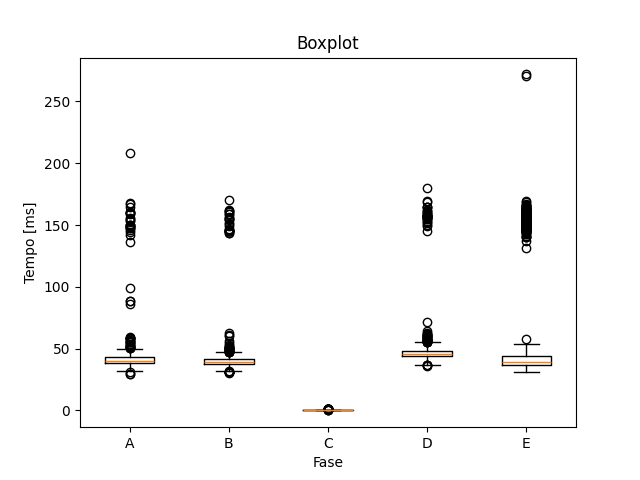
\includegraphics[width=\linewidth]{img/cap5/monolithic/boxplot.png}
		\end{subfigure}
		\begin{subfigure}{0.5\textwidth}
			\centering
			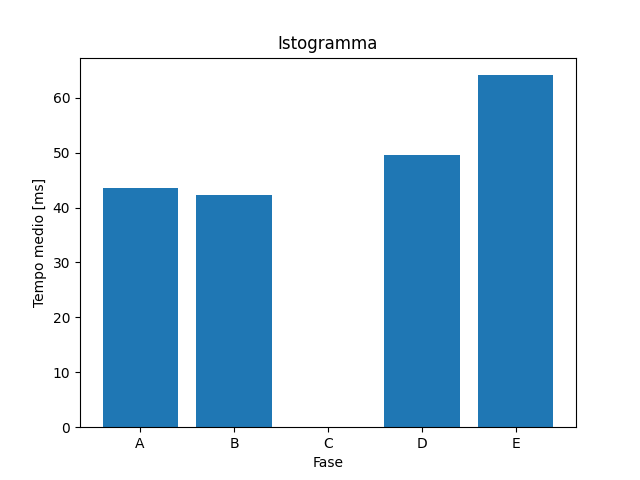
\includegraphics[width=\linewidth]{img/cap5/monolithic/istogramma.png}
		\end{subfigure}
		\caption{Boxplot e istogramma relativi ai tempi di esecuzione dell'applicazione monolitica}
		\label{fig:grafici-monolitica}
	\end{figure}
	
	\begin{figure}[tbp]
		\begin{subfigure}{0.5\textwidth}
			\centering
			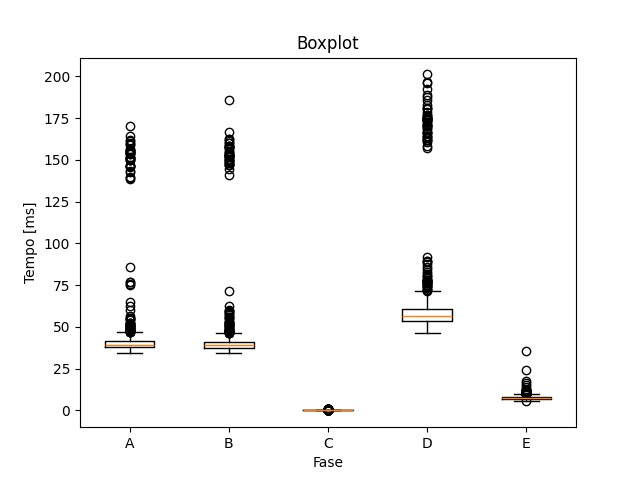
\includegraphics[width=\linewidth]{img/cap5/microservices/boxplot.png}
		\end{subfigure}
		\begin{subfigure}{0.5\textwidth}
			\centering
			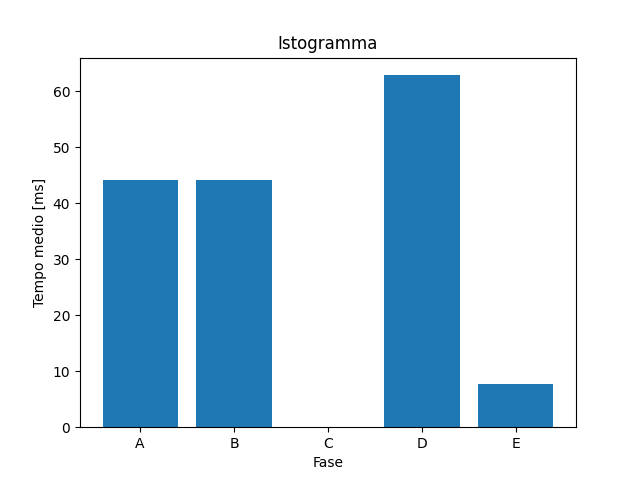
\includegraphics[width=\linewidth]{img/cap5/microservices/istogramma.png}
		\end{subfigure}
		\caption{Boxplot e istogramma relativi ai tempi di esecuzione dell'applicazione a microservizi}
		\label{fig:grafici-microserv}
	\end{figure}
	
	